\documentclass[reqno]{amsart}


\pagestyle{empty}

\usepackage{graphicx}
\usepackage[margin = 1cm]{geometry}
\usepackage{color}
\usepackage{cancel}
\usepackage{multirow}
\usepackage{framed}
\usepackage{algorithm}
\usepackage{algorithmic}
\usepackage{amssymb}
\usepackage{stackengine}
\usepackage{wrapfig}


\newtheorem{thm}{Theorem}
\newtheorem{cor}{Corollary}
\theoremstyle{definition}
\newtheorem{definition}{Definition}

\newenvironment{handwave}{%
  \renewcommand{\proofname}{Handwavey proof}\proof}{\endproof}
  %\renewcommand{\qedsymbol}{$\blacksquare$}

\begin{document}
\begin{flushleft}
{\sc \Large AMATH 301 Rahman} \hfill Week 9 Theory Part 1
\bigskip
\end{flushleft}

\newcommand{\R}{\mathbb{R}}
\newcommand{\N}{\mathbb{N}}
\newcommand{\Z}{\mathbb{Z}}
\newcommand{\Q}{\mathbb{Q}}
\renewcommand{\CancelColor}{\color{red}}
\newcommand{\?}{\stackrel{?}{=}}
\renewcommand{\varphi}{\phi}
\newcommand{\card}{\text{Card}}
\newcommand{\bigzero}{\text{\Huge 0}}
\newcommand{\curvearrowdown}{{\color{red}\rotatebox{90}{$\curvearrowleft$}}}
\newcommand{\curvearrowup}{{\color{red}\rotatebox{90}{$\curvearrowright$}}}



\section*{Week 9 Part 1:  Higher Order ODEs and Dynamical Systems}

\subsection*{Higher Order ODEs}

In the lecture I went over this kind of superficially, but here is all the gory detail.  If you want to skip to the more interesting stuff go to the next section.

Let us first go over some definitions we might not know,

\begin{definition}
An ODE is \underline{homogeneous} if it is of the form
\begin{equation}
p_n(t)y^{(n)}(t) + p_{n-1}(t)y^{(n-1)}(t) + \cdots + p_2(t)y''(t) + p_1(t)y'(t) + p_0(t)y(t) = 0.
\label{ODE}
\end{equation}
\end{definition}

So an example of a second order homogeneous ODE would be\\ $p_2y'' + p_1y' + p_0y = 0$.

\begin{definition}
An ODE is said to be \underline{nonhomogeneous} if it's not homogeneous.
\end{definition}

An example of a second order nonhomogeneous ODE would be $p_2y'' + p_1y' + p_0y = f(t)$.
In this section we will only deal with constant coefficients which mean each $p_n(t) = a_n$ where
$a_0, a_1, \ldots , a_{n-1}, a_n$ are all constants.

Now, we consider a special case of Eq. (\ref{ODE}): $y' + ay = 0$  We know how to solve this,
we simply use separation to get $y = ke^{-ax}$.  So, we can ``guess'' that the form of the
solutions for Eq. (\ref{ODE}) with constant coefficients will be $y = ke^{rx}$.  Now, we plug
this guess in to see what the solutions exactly are.  Notice that the nth derivative is,
$y^{(n)} = kr^ne^{rx}$, so plugging this into (\ref{ODE}) with $p_n(t) = a_n$ gives,
%
\begin{align*}
a_nkr^ne^{rx} + a_{n-1}kr^{n-1}e^{rx} + \cdots + a_2kr^2e^{rx} + a_1kre^{rx} + a_0ke^{rx} = 0\\
\Rightarrow ke^{rx}\left(a_nr^n + a_{n-1}r^{n-1} + \cdots + a_2r^2 + a_1r + a_0\right) = 0.
\end{align*}
%
Now, all we have to do is solve the polynomial equation.  Since this is an nth order polynomial,
there will be n solutions, i.e. $r = r_1, r_2, \ldots , r_{n-1}, r_n$.  Since the polynomial equation
has n solutions, the ODE will also have n solutions, so by superposition we get,
%
\begin{equation*}
y = k_1e^{r_1x} + k_2e^{r_2x} + \cdots + k_{n-1}e^{r_{n-1}x} + k_ne^{r_nx}.
\end{equation*}


We have just proved a theorem,

\begin{thm}
Consider the ODE
%
\begin{equation}
a_ny^{(n)}(x) + a_{n-1}y^{(n-1)}(x) + \cdots + a_2y''(x) + a_1y'(x) + a_0y(x) = 0.
\label{ODE2}
\end{equation}
%
such that $a_0, a_1, \ldots , a_{n-1}, a_n$ are constants.  Then,
%
\begin{equation}
y = k_1e^{r_1x} + k_2e^{r_2x} + \cdots + k_{n-1}e^{r_{n-1}x} + k_ne^{r_nx},
\end{equation}
%
where $k_1, k_2, \ldots , k_{n-1}, k_n$ are constants and $r_1, r_2, \ldots , r_{n-1}, r_n$
satisfy the polynomial equation
%
\begin{equation}
a_nr^n + a_{n-1}r^{n-1} + \cdots + a_2r^2 + a_1r + a_0 = 0,
\label{charpoly}
\end{equation}
%
only if $r_1 \neq r_2 \neq \cdots \neq r_{n-1} \neq r_n$.
\end{thm}

\begin{definition}
We call Eq. (\ref{charpoly}) the \underline{characteristic equation} of ODE (\ref{ODE2}),
and the polynomial is called the \underline{characteristic polynomial}.
\end{definition}

\pagebreak

Now, lets do a few problems,

\begin{enumerate}

\item[Ex:  ]  $y'' + 2y' - 3y = 0$

\textbf{Solution:  }
  The characteristic polynomial is $r^2 + 2r - 3$, so
%
\begin{equation*}
r^2 + 2r - 3 = 0 \Rightarrow (r+3)(r-1) = 0 \Rightarrow r = 1, -3 \Rightarrow y = c_2e^x + c_2e^{-3x}.
\end{equation*}
%

\item[Ex:  ]  $y'' - 9y' + 9 = 0$

\textbf{Solution:  }
The characteristic polynomial is $r^2 - 9r + 9$, so
%
\begin{equation*}
r = \frac{1}{2}(9 \pm 3\sqrt{5}) \Rightarrow y = c_1e^{\frac{1}{2}(9 + 3\sqrt{5})x} +  c_2e^{\frac{1}{2}(9 - 3\sqrt{5})x}.
\end{equation*}
%

\item[Ex:  ] $y'' + 3y' = 0;\; y(0) = -2,\, y'(0) = 3$

\textbf{Solution:  }
 The characteristic polynomial is $r^2 + 3r$, so
%
\begin{equation*}
r = 0, -3 \Rightarrow y = c_1 + c_2e^{-3x},
\end{equation*}
%
and from the initial conditions we get $y = -1-e^{-3x}$.

\item[Ex:  ]  

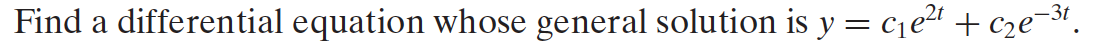
\includegraphics[width = 0.9\textwidth]{BoyceDiPrima_pg144_Ex18}

\textbf{Solution:  }
Here they give us the solution and we have to extract the ODE.
Notice that from the solution we deduce 
%
\begin{equation*}
r = -\frac{1}{2}, -2 \Rightarrow (r+\frac{1}{2})(r+2) = r^2 + \frac{5}{2}r+1 = 0
\Rightarrow y'' + \frac{5}{2}y' + y = 0.
\end{equation*}
%

\item[Ex:  ]  

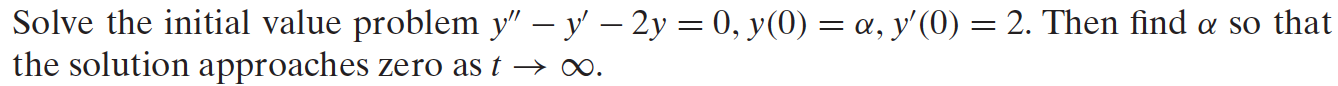
\includegraphics[width = 0.9\textwidth]{BoyceDiPrima_pg144_Ex21}

\textbf{Solution:  }
This is kind of a silly question, but since there is a similar one on the homework lets do it.
We solve the ODE as per usual,
%
\begin{equation*}
r^2 - r - 2 = (r-2)(r+1) = 0 \Rightarrow r = -1, 2 \Rightarrow y = c_1e^{-x} + c_2e^{2x}.
\end{equation*}
%
From the initial condition we have the equations $c_1 + c_2 = \alpha$ and $2c_2 - c_1 = 2$,
so $3c_2 = \alpha + 2$.  This means that if $\alpha = -2$, as $t \rightarrow \infty$, $y \rightarrow 0$.
However, for the second part of the problem there are no solutions that always blow up because we have
a negative exponential term that will persist.

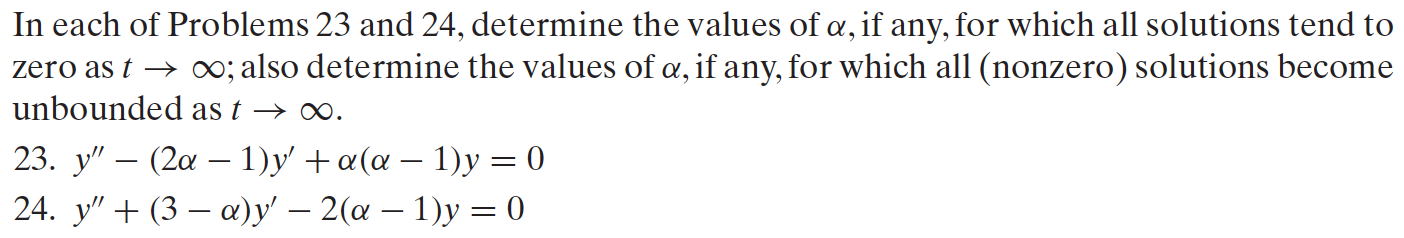
\includegraphics[width = 0.9\textwidth]{BoyceDiPrima_pg144_Ex24}

\item[24)]  For this problem the ODE itself has the parameter $\alpha$.  This leads
to interesting conclusions without even solving, but the easiest most intuitive way
to come to those conclusions will be by solving, even though it is more tedious and time consuming.
We solve the ODE,
%
\begin{equation*}
r^2 + (3 - \alpha)r - 2(\alpha - 1) = 0 \Rightarrow (r-(\alpha - 1))(r+2) = 0 \Rightarrow r = -2, \alpha - 1
\Rightarrow y = c_2e^{-2x} + c_2e^{(\alpha - 1)x}.
\end{equation*}
%
So, for $\alpha < 1$, $y \rightarrow \infty$.  If $\alpha = 1$, $y \rightarrow c_2$,
and if $\alpha > 1$, and $y \rightarrow \pm \infty$ only if $c_2 \neq 0$.

\end{enumerate}

\pagebreak

\subsection*{Dynamical Systems}

\begin{wrapfigure}[]{R}{0.35\textwidth}
\centering
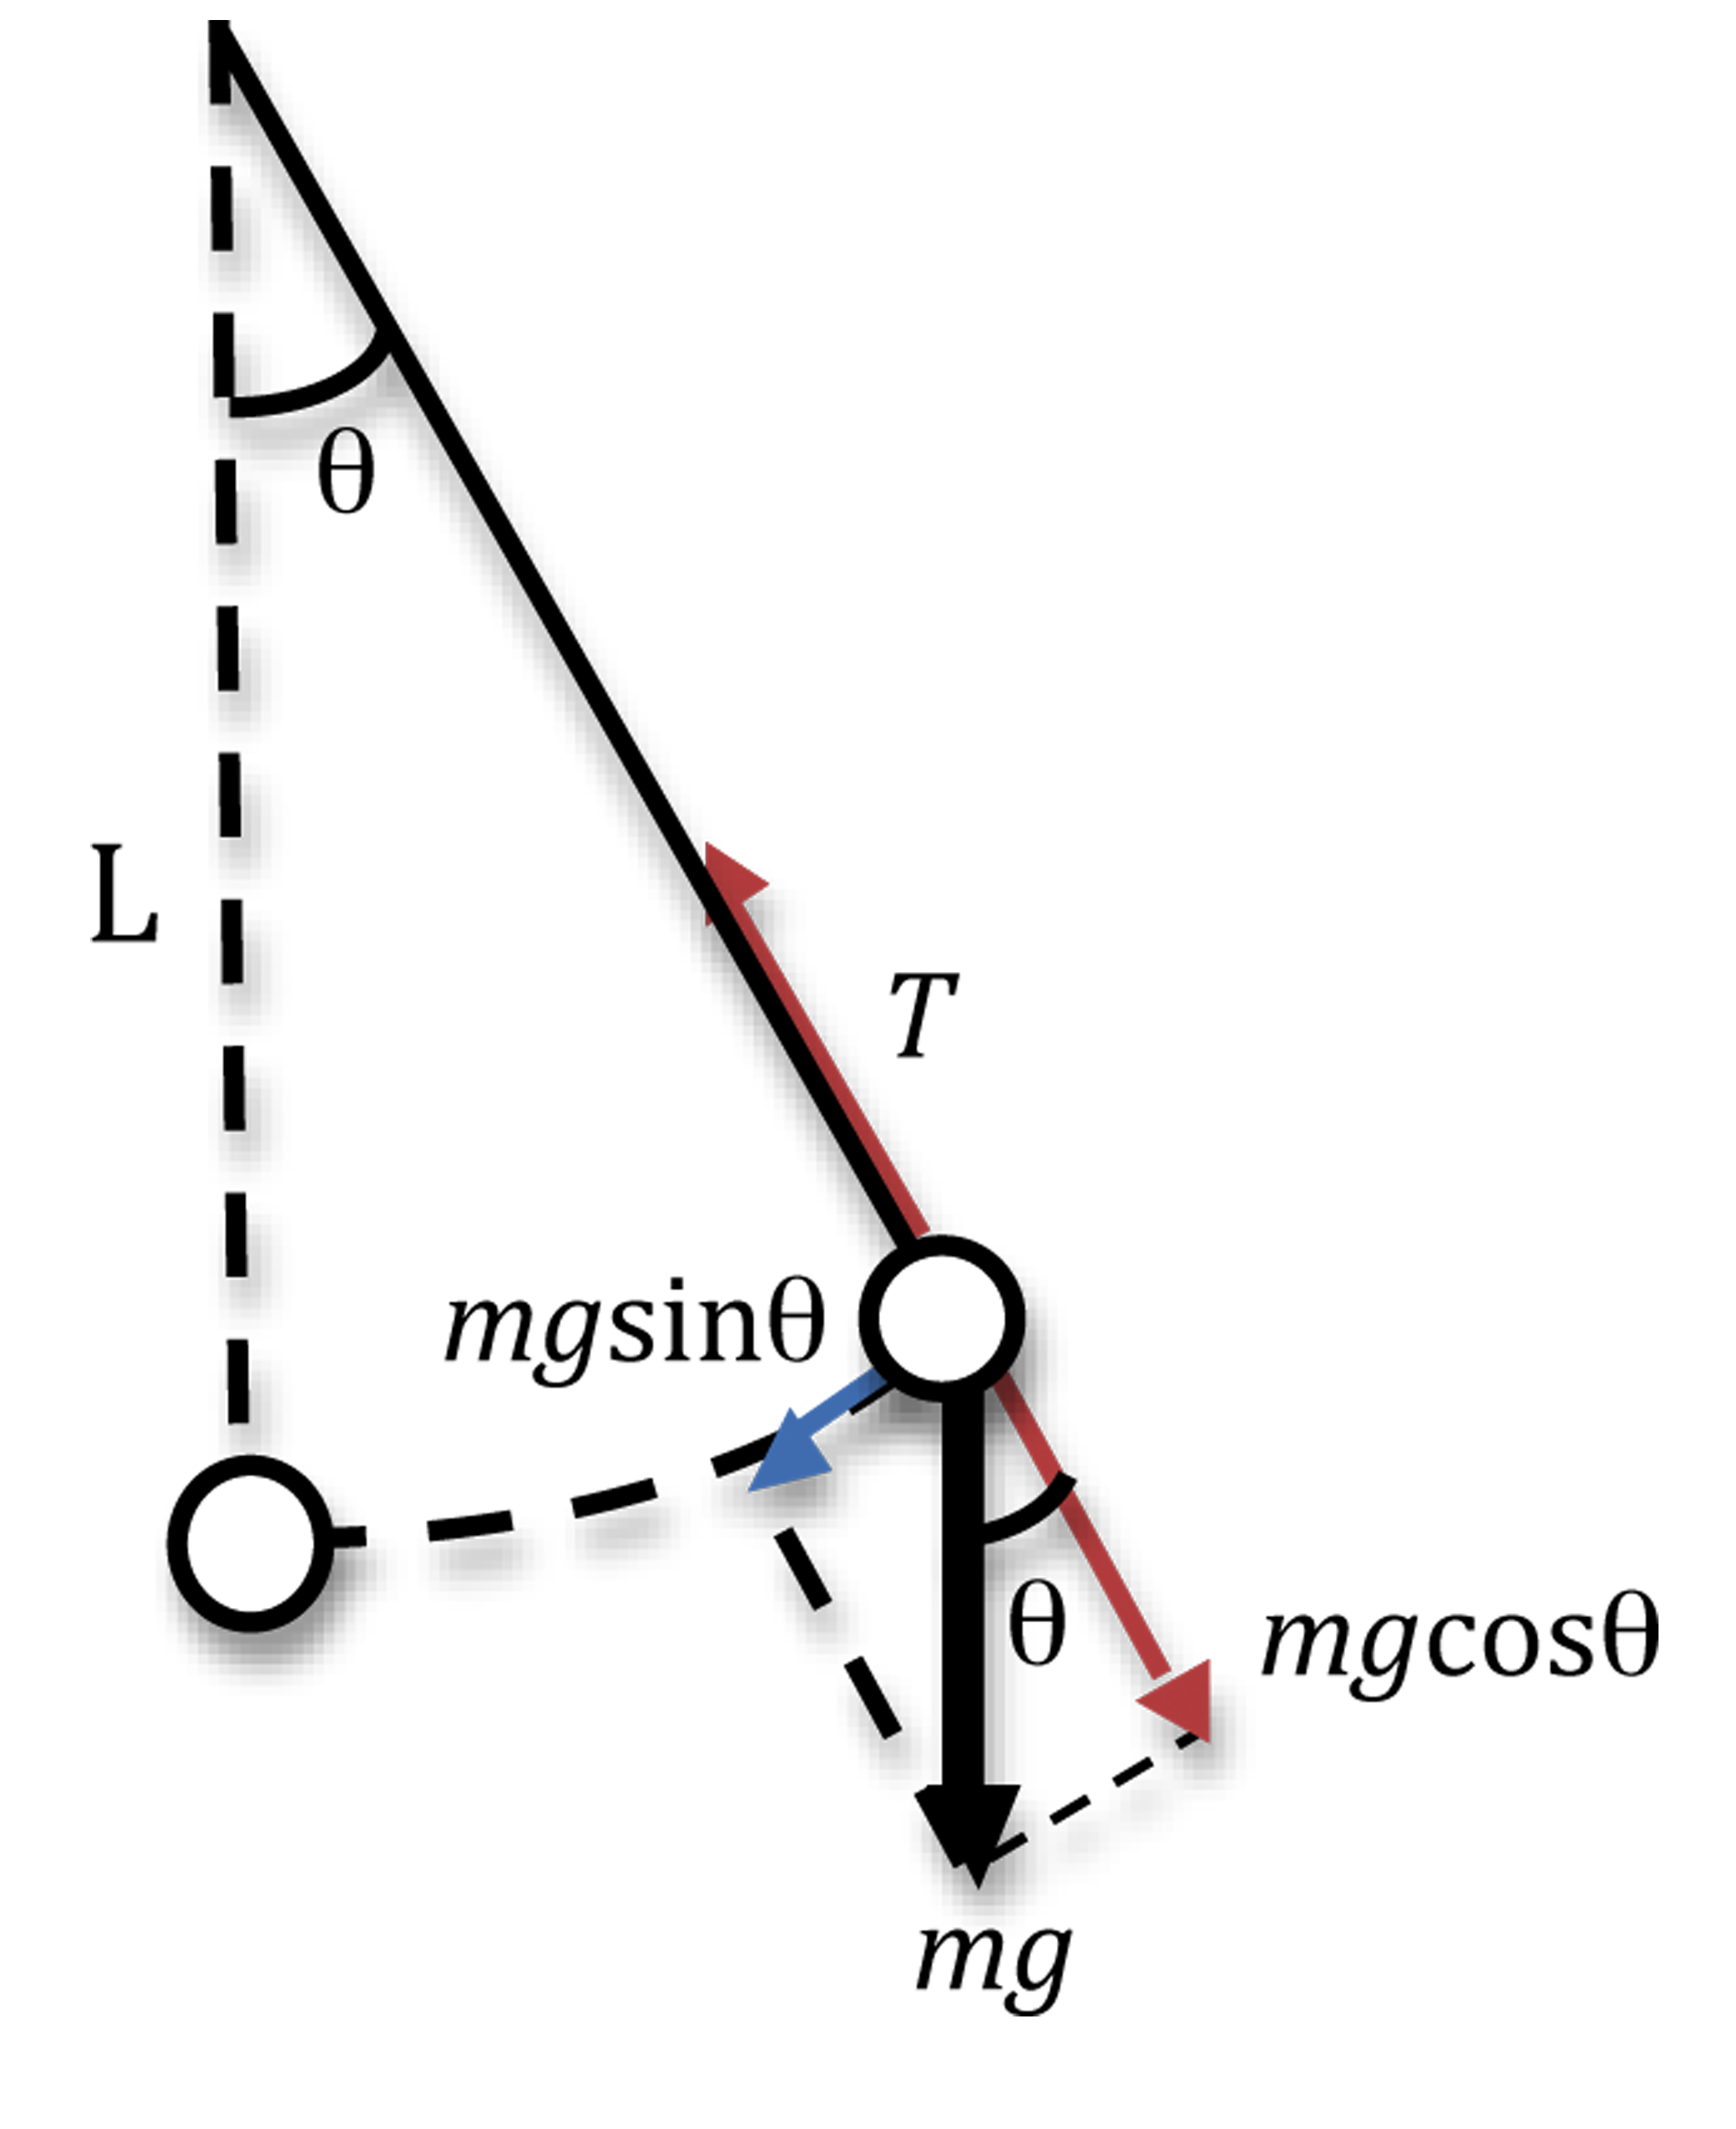
\includegraphics[width = 0.33\textwidth]{Pendulum}
\end{wrapfigure}

Sometimes we just can't solve problems exactly.  In fact most problems don't have exact solutions.
These equations are either solved numerically, in which case the numerics might get it wrong, or
we extract information form the equations without solving.

Consider the pendulum.  We will consider both the frictional and frictionless case.  \textbf{For the exam
just to keep things simple we will just focus on the frictionless case}, but it is important to understand
what happens in the frictional case as well.

In order to derive the ODE we need the force along its arc.  Then we use Newton's law: $F = ma$.
To find the acceleration $a$ along the arc lets consider the arc length: $s = L\theta$, then
the velocity is $v = L\frac{d\theta}{dt} = \dot{\theta}$, and the acceleration is
$a = L\frac{d^2\theta}{dt^2} = \ddot{\theta}$, which gives us a force of $F = m\ddot{\theta}$.
Now we need to figure out what $F$ is.  This consists of the force from gravitational acceleration
and damping from friction, $F = -\nu L\dot{\theta} - mg\sin\theta$.  This gives us the ODE
%
\begin{equation*}
mL\frac{d^2\theta}{dt^2} = -\nu L\frac{d\theta}{dt} - mg\sin\theta
\Rightarrow \frac{d^2\theta}{dt^2} + \frac{\nu}{m}\frac{d\theta}{dt} + \frac{g}{L}\sin\theta = 0
\end{equation*}
%
But this is really ugly, so lets simplify the equation a bit,
%
\begin{equation}
\ddot{\theta} = -\gamma \dot{\theta} - k\sin\theta
\end{equation}
%
Higher order equations are tough to deal with, especially when they are nonlinear, so lets
change this into a system of first order equations by letting $\omega = \dot{\theta}$
%
\begin{equation*}
\begin{split}
\dot{\theta} &= \omega\\
\dot{\omega} &= -\gamma\omega - k\sin\theta
\end{split}
\end{equation*}
%
We can't change this into a matrix equation because it is nonlinear.  However, we can use similar
techniques after linearizing about special solutions called \emph{fixed points} (f.p.'s) $(\theta_*,\omega_*)$, which
are points for which the object isn't moving; i.e. $\dot{\omega} = 0$ and $\dot{\theta} = 0$.
This means we set the right hand side (RHS) to zero
%
\begin{equation*}
\dot{\theta_*} = 0 \Rightarrow \omega_* = 0 \Rightarrow \dot{\omega_*} = -\gamma\cancelto{0}{\omega}_*
-k\sin\theta_* = 0 \Rightarrow \theta_* = n\pi;\; n\in \Z \Rightarrow (\theta_*,\omega_*) = (n\pi,0)
\end{equation*}
%
Now we can linearlize about these fixed points.  In order to do this we will use the \emph{Jacobian}
also known as the derivative matrix in 2-D.
%
\begin{equation}
J(\theta_*,\omega_*) = \begin{pmatrix}
\dfrac{\partial f}{\partial\theta} & \dfrac{\partial f}{\partial \omega}\\
\dfrac{\partial g}{\partial \theta} & \dfrac{\partial g}{\partial \omega}
\end{pmatrix}_{(\theta_*,\omega_*)}
\end{equation}
%
For our case this will be
%
\begin{equation}
J(n\pi,0) = \begin{pmatrix}
0 & 1\\
-k\cos\theta & -\gamma
\end{pmatrix}_{(n\pi,0)} = \begin{pmatrix}
0 & 1\\
\mp k & -\gamma
\end{pmatrix} \text{  for $n$ even and odd, respectively.}
\label{Eq: Jacobian}
\end{equation}
%

Intuitively we know that we are going to get different solutions for the frictional and frictionless case.
Lets first do the frictionless case.

\subsection*{Frictionless Case $(\gamma = 0)$}  Here the fixed points are the same, but now
our Jacobian is going to be slightly different
%
\begin{equation}
J(n\pi,0) = \begin{pmatrix}
0 & 1\\
-k\cos\theta & 0
\end{pmatrix}_{(n\pi,0)} = \begin{pmatrix}
0 & 1\\
\mp k & 0
\end{pmatrix} \text{  for $n$ even and odd, respectively.}
\end{equation}
%
Then we look for the eigenvalues for our two fixed point cases.

\underline{\Large $n$ even.}  When $n$ is even we have
%
\begin{equation}
\begin{vmatrix}
-\lambda & 1\\
-k & -\lambda
\end{vmatrix} = 0 \Rightarrow \lambda^2 = -k \Rightarrow \lambda = \pm\sqrt{-k} = \pm i\sqrt{k}
\end{equation}
%
This is what's called a \emph{center} fixed point, and this admits oscillatory solutions since we have
complex conjugate eigenvalues without a real part; i.e. pure sines and cosines.

\underline{\Large $n$ odd.}  When $n$ is odd we have
%
\begin{equation}
\begin{vmatrix}
-\lambda & 1\\
k & -\lambda
\end{vmatrix} = 0 \Rightarrow \lambda^2 = k \Rightarrow \lambda = \pm\sqrt{k}
\end{equation}
%
This is called a \emph{saddle} fixed point, and this admits exponentially decaying solutions in
one direction and exponentially expanding solutions in the other direction.

Now we can sketch what's called a \emph{phase portrait} also called a \emph{phase plane diagram}.
This is a vector field in $(\theta,\omega)$ space.  This is a way we can visualize how the position
and velocity of solutions are related.  The phase portrait for the frictionless pendulum is going to look
as such
%
\begin{figure}[htbp]
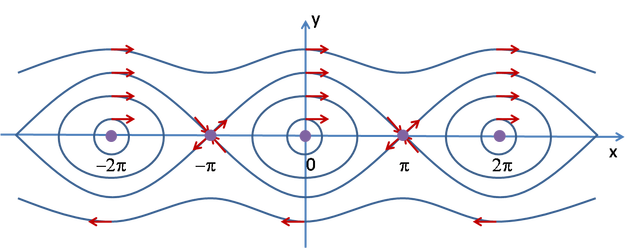
\includegraphics[width = \textwidth]{pendulum-portrait}
\end{figure}
%
When two saddle fixed points are connected it is called a \emph{heteroclinic orbit}.
And if a saddle is connected to itself it's called a \emph{homoclinic orbit}.
%

\subsection*{Frictional Case $(\gamma > 0)$}  Now lets look at the frictional case.
For this case I won't sketch the full phase portrait.  I will just show the local vector
field around the fixed point just so I can define the various types of stability.
From \eqref{Eq: Jacobian} we have two cases of $n$.  Lets first look at the odd $n$'s

\underline{\Large $n$ odd.}  When $n$ is odd we have
%
\begin{equation}
\begin{vmatrix}
-\lambda & 1\\
 k & -\gamma - \lambda
\end{vmatrix} = \lambda^2 + \gamma \lambda - k = 0 \Rightarrow \lambda
= \frac{1}{2}\left(-\gamma \pm \sqrt{\gamma^2 + 4k}\right).
\end{equation}
%
Notice that the discriminant here is always positive, also $\sqrt{\gamma^2 + 4k} > \gamma$,
which means for $+\sqrt{\gamma^2 + 4k}$ it is exponentially expanding and for
$-\sqrt{\gamma^2 + 4k}$ it is exponentially decaying.  So the fixed point when $n$ is odd
is a \emph{saddle} fixed point.  We already know the sketch of a saddle so I won't sketch it here.

\underline{\Large $n$ even.}  When $n$ is even we have
%
\begin{equation}
\begin{vmatrix}
-\lambda & 1\\
 -k & -\gamma - \lambda
\end{vmatrix} = \lambda^2 + \gamma \lambda + k = 0 \Rightarrow \lambda
= \frac{1}{2}\left(-\gamma \pm \sqrt{\gamma^2 - 4k}\right).
\end{equation}
%
Notice that this has two cases.  Either the discriminant is negative or positive.

\begin{wrapfigure}[]{R}{0.4\textwidth}
\centering
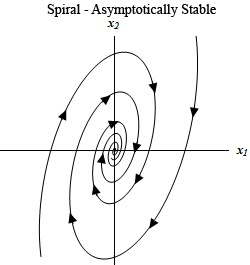
\includegraphics[width = 0.19\textwidth]{StableSpiral}
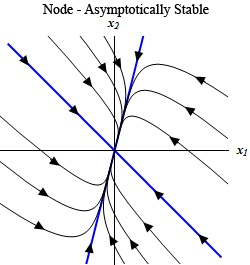
\includegraphics[width = 0.19\textwidth]{StableNode}
\end{wrapfigure}

\underline{\large $\gamma^2 - 4k < 0$.}  For this case we get complex conjugate
eigenvalues, but notice that the real part is negative.  This means we will get
decaying oscillatory solutions, and the fixed point is called a \emph{stable spiral}.

\underline{\large $\gamma^2 - 4k > 0$.}  For this case we get negative real solutions
since $\sqrt{\gamma^2 - 4k} < \gamma$.  This means we get decaying solutions,
and the fixed point is called a \emph{stable node}.

\subsection*{Forced Case $(\gamma < 0)$}  There is one more case.  What if
$\gamma$ is negative.  Then this isn't damped anymore, it's actually forced.
We still have the even and odd cases, but now the real part will always be
positive.

\underline{\Large $n$ odd.}  When $n$ is odd we have a saddle fixed point
again since we have both positive and negative real eigenvalues because $\sqrt{\gamma^2 + 4k} > \gamma$,
so for $+\sqrt{\gamma^2 + 4k}$ it is exponentially expanding and for
$-\sqrt{\gamma^2 + 4k}$ it is exponentially decaying.

\underline{\Large $n$ even.}  When $n$ is even we have the same positive
or negative discriminant, except now we have positive real parts.

\begin{wrapfigure}[]{R}{0.4\textwidth}
\centering
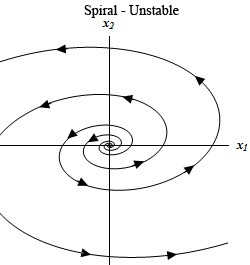
\includegraphics[width = 0.19\textwidth]{UnstableSpiral}
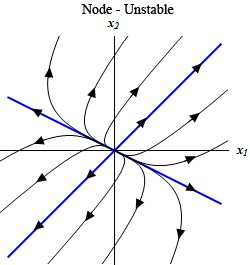
\includegraphics[width = 0.19\textwidth]{UnstableNode}
\end{wrapfigure}

\underline{\large $\gamma^2 - 4k < 0$.}  For this case we get complex conjugate
eigenvalues, but notice that the real part is positive.  This means we will get
expanding oscillatory solutions, and the fixed point is called an \emph{unstable spiral}.

\underline{\large $\gamma^2 - 4k > 0$.}  For this case we get positive real solutions
since $\sqrt{\gamma^2 - 4k} < \gamma$.  This means we get expanding solutions,
and the fixed point is called an \emph{unstable node}.

\subsection*{Summary}

We can summarize all of this in this table.  There are other cases called \emph{borderline}
cases, but lets not worry about that for this class.

\begin{table}[htbp]
\centering
\begin{tabular}{c||c|c|}
Case & Eigenvalue & Description\\
\hline
Stable Node & $\lambda_{1,2} < 0$ & Exponential Decay\\
\hline
Unstable Node & $\lambda_{1,2} > 0$ & Exponential Expansion\\
\hline
Stable Spiral & $\lambda_{1,2} = \xi \pm i\theta$ where $\xi < 0$ & Oscillatory Decay\\
\hline
Unstable Spiral & $\lambda_{1,2} = \xi \pm i\theta$ where $\xi > 0$ & Oscillatory Expansion\\
\hline
Center & $\lambda_{1,2} = \pm i\theta$ & Pure Oscillations\\
\hline
Saddle & $\lambda_1 < 0$ and $\lambda_2 > 0$ & Exponential Decay in one direction\\
& & and Exponential Expansion in the other\\
\hline
\end{tabular}
\end{table}

\begin{figure}[htbp]
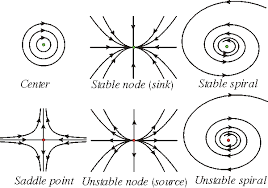
\includegraphics[width = 0.5\textwidth]{Summary}
\end{figure}

And here is another picture of the the types of fixed points when they don't line up perfectly with the axes:

\begin{figure}[htbp]
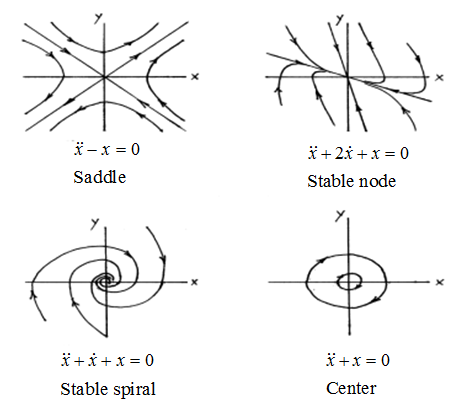
\includegraphics[width = 0.5\textwidth]{Summary1}
\end{figure}

\begin{enumerate}

\item[Ex:  ]  Lets do a couple of really simple example that you will definitely not see on the exam
just to solidify some concepts.  These concepts in 1-D will expand to 2-D, but in 1-D we only have
three cases, whereas in 2-D we have six main cases and three borderline cases.  In this class we won't
go over borderline cases.

\begin{enumerate}

\item  Consider $\frac{dx}{dt} = \dot{x} = f(x) = -x$.  Clearly the fixed point is $x=0$, but is it stable or
unstable?  Well, if $x > 0$ the ODE will pull it back to zero, and if $x < 0$ it will also go back to zero.
So this fixed point is \emph{stable}.  Another way we can show this is by taking the derivative,
$f'(x_* = 0) = -1 < 0$.

\item  Now consider $\frac{dx}{dt} = \dot{x} = f(x) = x$.  The fixed point is $x = 0$ again, but
now it's \emph{stable} since a point starting off the fixed point will want to go away from it.  Also,
$f'(x_* = 0) = 1 > 0$.

\item  We can also have something that is bi-stable.  Consider $\frac{dx}{dt} = \dot{x} = f(x) = x^2$.
Then for $x > 0$ the trajectory diverges from zero, but for $x < 0$ the trajectory goes towards zero.
We'll notice that $f'(x_* = 0) = 0$, so linear stability analysis fails here; i.e. the derivative test is not
enough to tell us anything about stability.  Notice that $\frac{dx}{dt} = \dot{x} = f(x) = x^3$, also
has a fixed point at zero with a zero derivative, but this is stable.

\end{enumerate}

\item[Ex:  ]  Now lets look at a 2-D example with linear equations.  Fun fact: this is a model for
love affairs written by Strogatz 1988.
%
\begin{equation}
\begin{split}
\dot{x} &= ax + by\\
\dot{y} &= bx + ay
\end{split}; \qquad a < 0,\, b>0
\end{equation}
%
Lets first find the fixed points: $ax_* + by_* = 0;\; cx_* + dy_* = 0 \Rightarrow x_* = y_* = 0$.
You can convince yourself of this by either Gaussian elimination or simultaneous equations.
Then we find the eigenvalues
%
\begin{equation*}
J(x_*,y_*) = \begin{vmatrix}
a & b\\
b & a
\end{vmatrix} \Rightarrow \begin{vmatrix}
a - \lambda & b\\
b & a - \lambda
\end{vmatrix} = \lambda^2 - 2a\lambda + a^2 - b^2 = 0
\Rightarrow \lambda = \frac{1}{2}\left(2a \pm \sqrt{4a^2 - 4a^2 + 4b^2}\right) = a \pm b.
\end{equation*}
%
Since $a < 0$ and $b > 0$ we have two cases:
%
$|a| > |b|$:  $\lambda_{1,2} < 0$ and $|a| < |b|$:  $\lambda_1 = a - b < 0$, $\lambda_2 = b - a > 0$.
These two cases are illustrated in the figures below (left).  Now, we could use eigenvectors to get the precises
direction of the trajectories, but these problems are simple enough that we can forgo using eigenvectors
and just think of the vector field near the fixed point.
%
\begin{figure}[htbp]
\centering
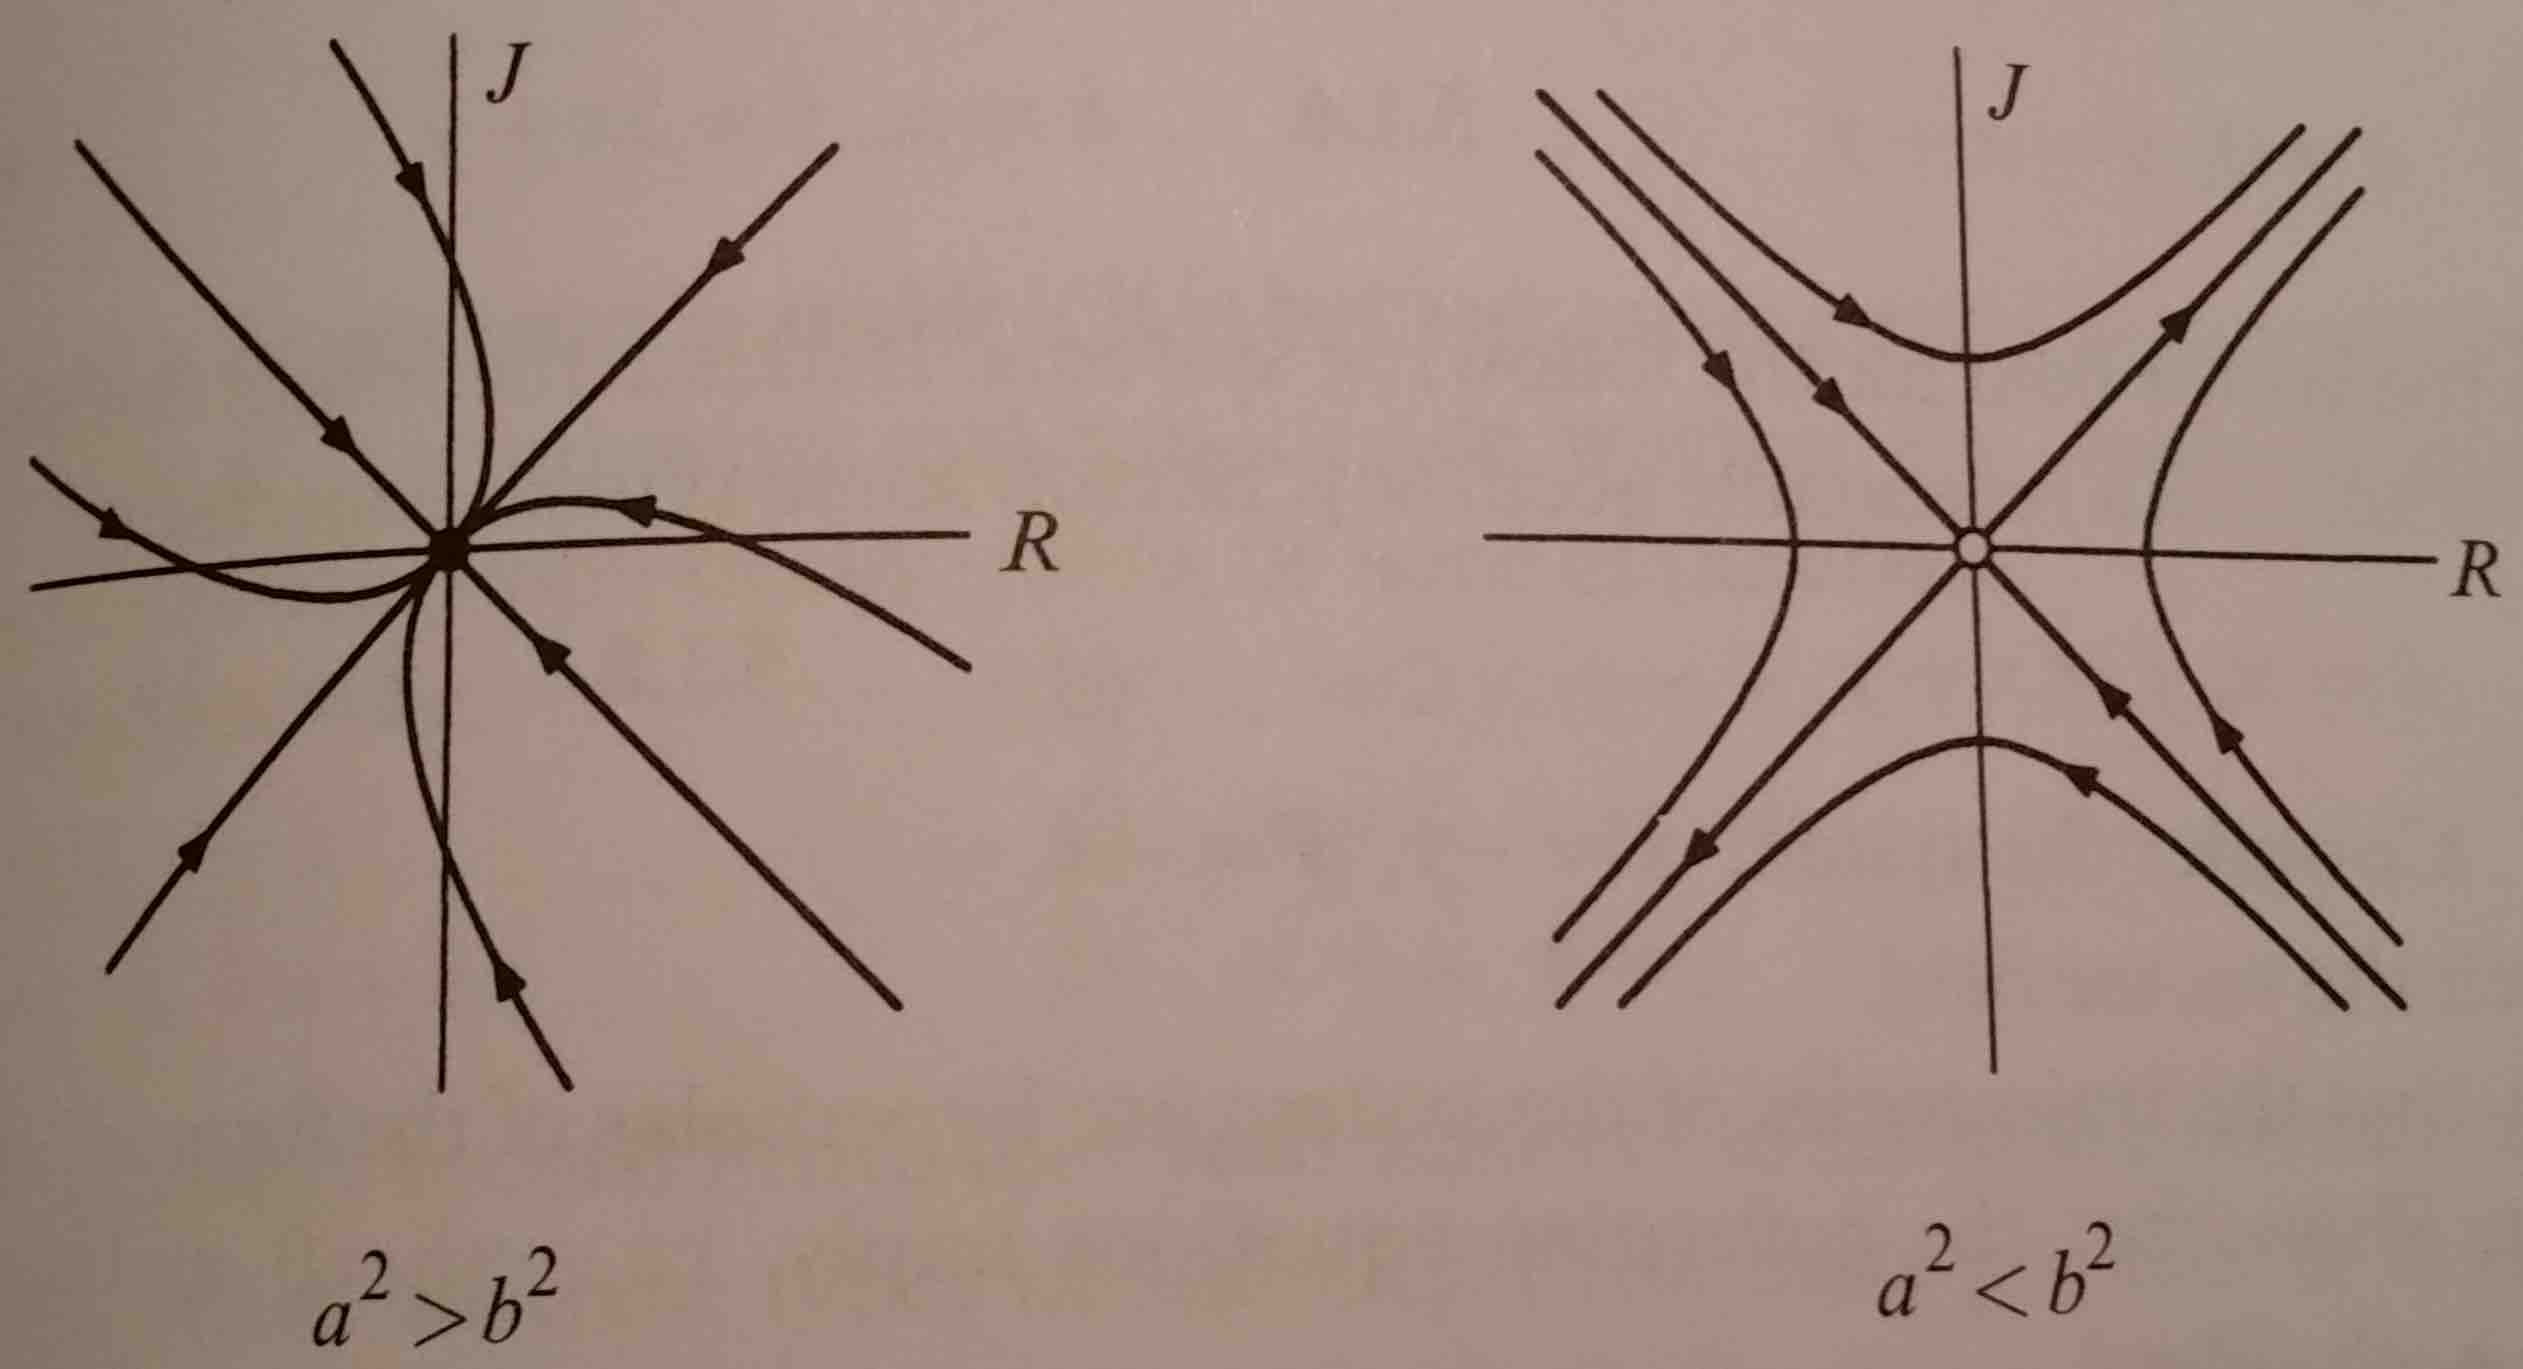
\includegraphics[width = 0.668\textwidth]{Love1}
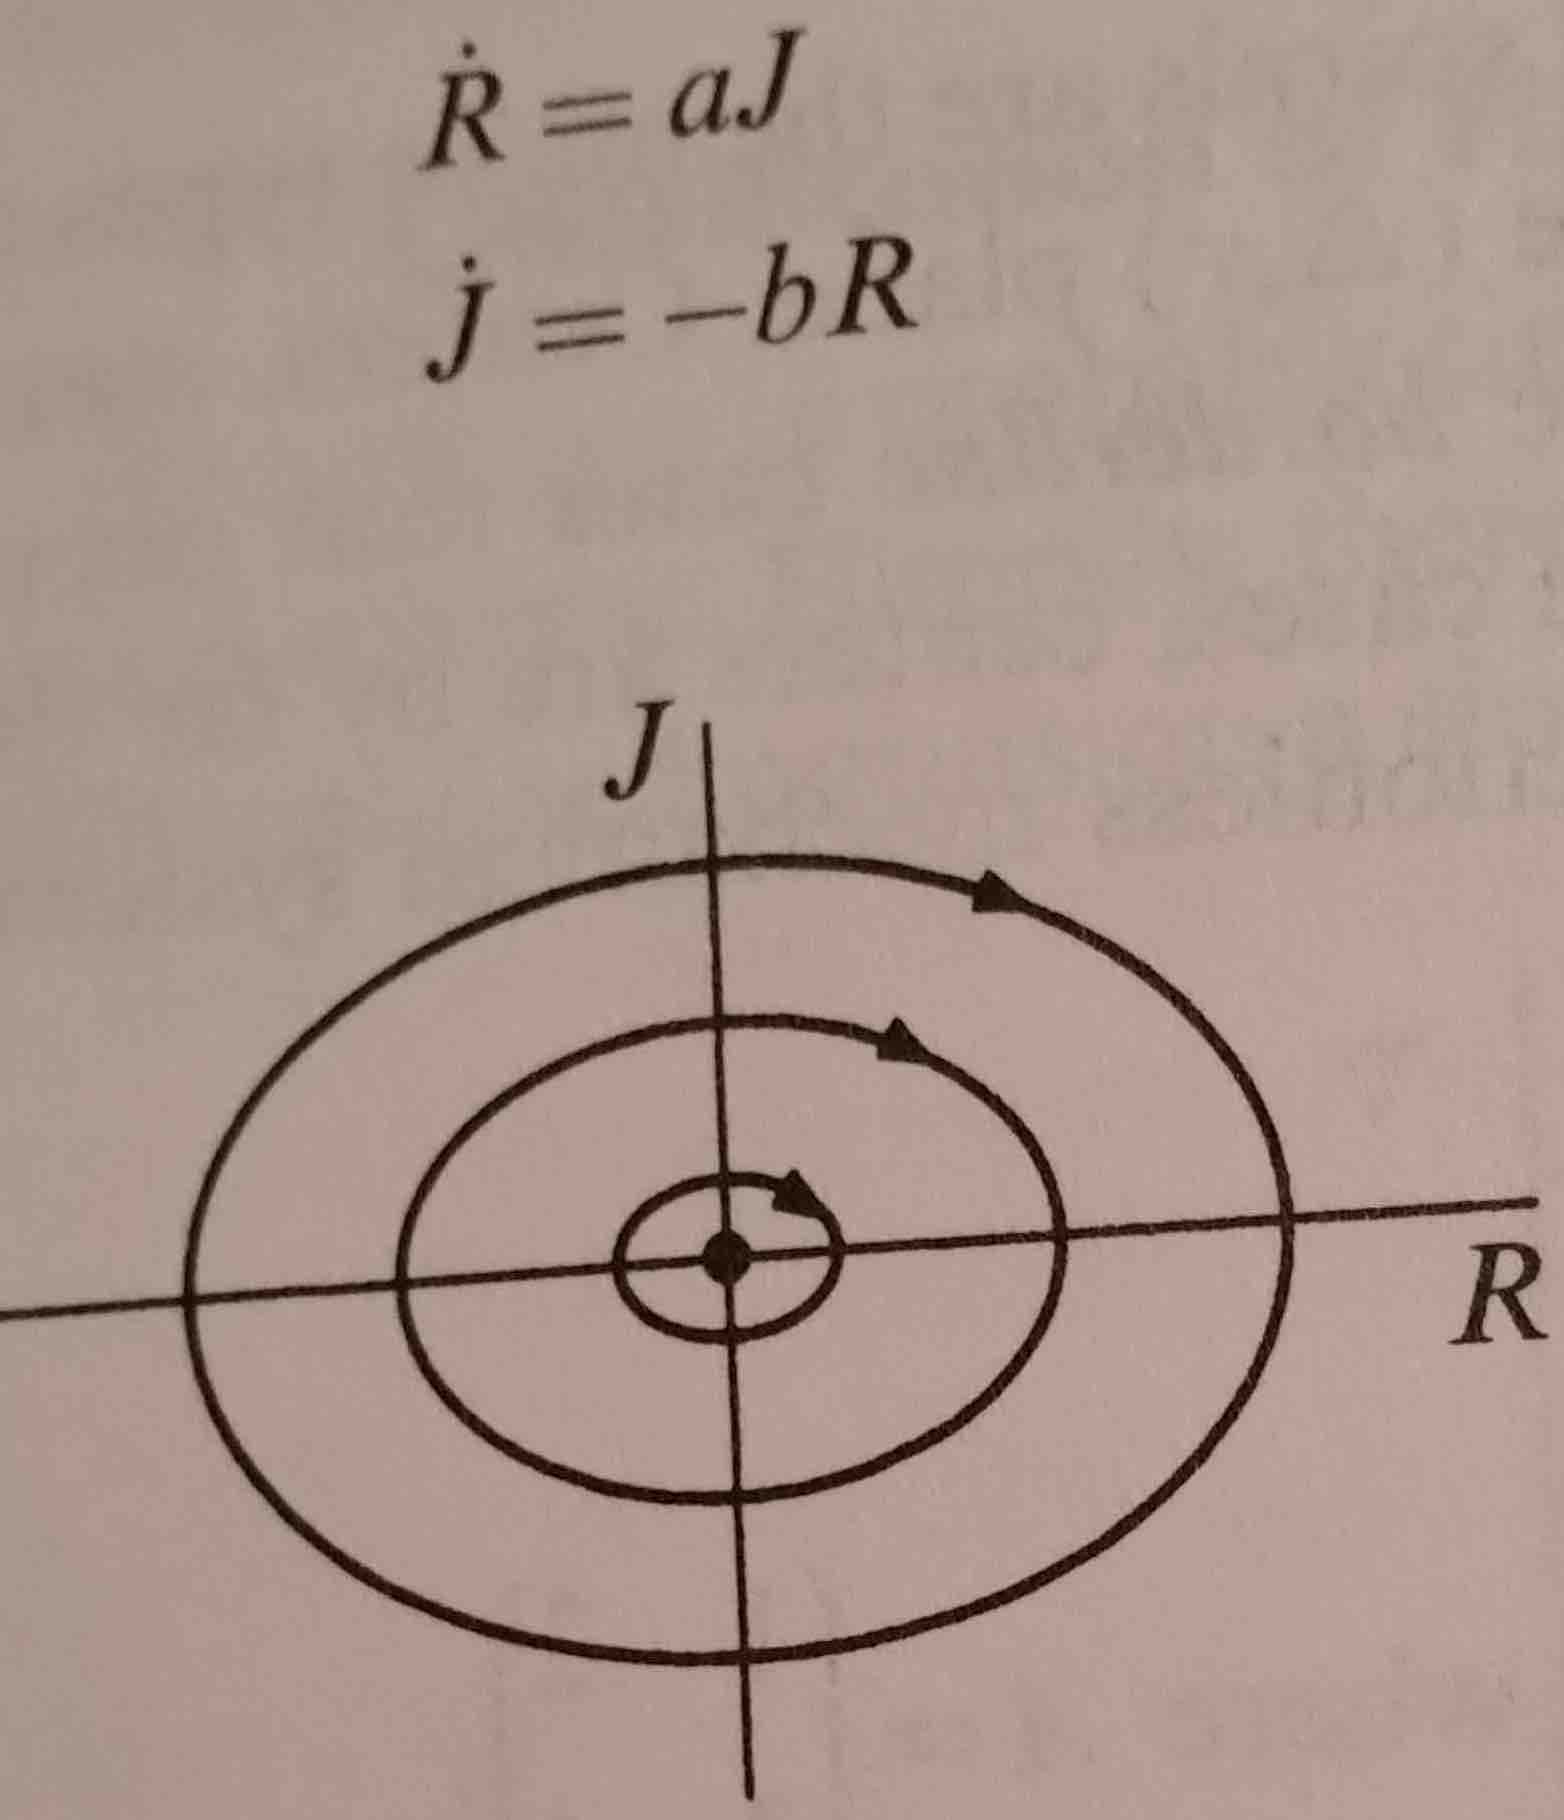
\includegraphics[width = 0.312\textwidth]{Love2}
\end{figure}
%
\item[Ex:  ]  Lets look at a simpler version of the above equation
%
\begin{equation}
\begin{split}
\dot{x} &= ay\\
\dot{y} &= -bx
\end{split};\qquad a,b > 0
\end{equation}
%
Clearly the fixed point is $(x_*,y_*) = (0,0)$.  For the eigenvalues we have
%
\begin{equation*}
J(x_*,y_*) = \begin{vmatrix}
0 & a\\
-b & 0
\end{vmatrix} \Rightarrow \begin{vmatrix}
- \lambda & a\\
-b & - \lambda
\end{vmatrix} = \lambda^2 + ab = 0 \Rightarrow \lambda = \pm i\sqrt{ab}.
\end{equation*}
%
So this fixed point is a center with the phase portrait on the right.

\item[Ex:  ]  Here is a concrete example somewhat similar to the one on the exam, except
this problem is actually more difficult than the one that will be on the exam.  The problem
is exactly the way it will look on the exam except with a different ODE, so hope it helps.

Consider the ODE
%
\begin{equation}
\begin{split}
\dot{x} &= y\\
\dot{y} &= x - x^3
\end{split}
\end{equation}

\begin{enumerate}

\item  Find all fixed points.

\textbf{Solution:  }  $\dot{x}_* = 0 \Rightarrow y_* = 0$ and
$\dot{y}_* = 0 \Rightarrow x_* - x_*^3 = x_*(1 - x_*^2) = x_*(1-x_*)(1+x_*) = 0 \Rightarrow x_* = 0, \pm 1$,
so the three fixed points are $(x_*,y_*) = (0,0),\,(-1,0),\,(1,0)$.

\item  Linearize about the fixed points.

\textbf{Solution:  }  First we compute the Jacobian,
%
\begin{equation*}
J(x_*,y_*) = \begin{pmatrix}
0 & 1\\
1-3x_*^2 & 0
\end{pmatrix} \Rightarrow J(0,0) = \begin{pmatrix}
0 & 1\\
1 & 0
\end{pmatrix}; \qquad J(\pm 1,0) = \begin{pmatrix}
0 & 1\\
-2 & 0
\end{pmatrix}
\end{equation*}

\item  Find the eigenvalues of the linearized system.

\textbf{Solution:  }  For $(x_*,y_*) = (0,0)$ we have
%
\begin{equation*}
\begin{vmatrix}
-\lambda & 1\\
1 & -\lambda
\end{vmatrix} = \lambda^2 -1 = 0 \Rightarrow \lambda = \pm 1
\end{equation*}
%
And for $(x_*,y_*) = (\pm 1,0)$ we get
%
\begin{equation*}
\begin{vmatrix}
-\lambda & 1\\
-2 & -\lambda
\end{vmatrix} = \lambda^2 + 2 = 0 \Rightarrow \lambda = \pm i\sqrt{2}
\end{equation*}

\item  State the stability of each fixed point.

\textbf{Solution:  }  $(x_*,y_*) = (0,0)$ is a \underline{saddle} fixed point since $\lambda_1 = -1 < 0$
and $\lambda_2 = 1 > 0$.  $(x_*,y_*) = (\pm 1,0)$ are \underline{centers} since $\lambda$ is a complex
conjugate with zero real part.

\item  Sketch the phase portrait.

\textbf{Solution:  }  This has a homoclinic orbit unlike in the pendulum that had a heteroclinic orbit, because there
is only one saddle point and the trajectory comes out of the saddle point back into the saddle point.
The figure is below:
%
\begin{figure}
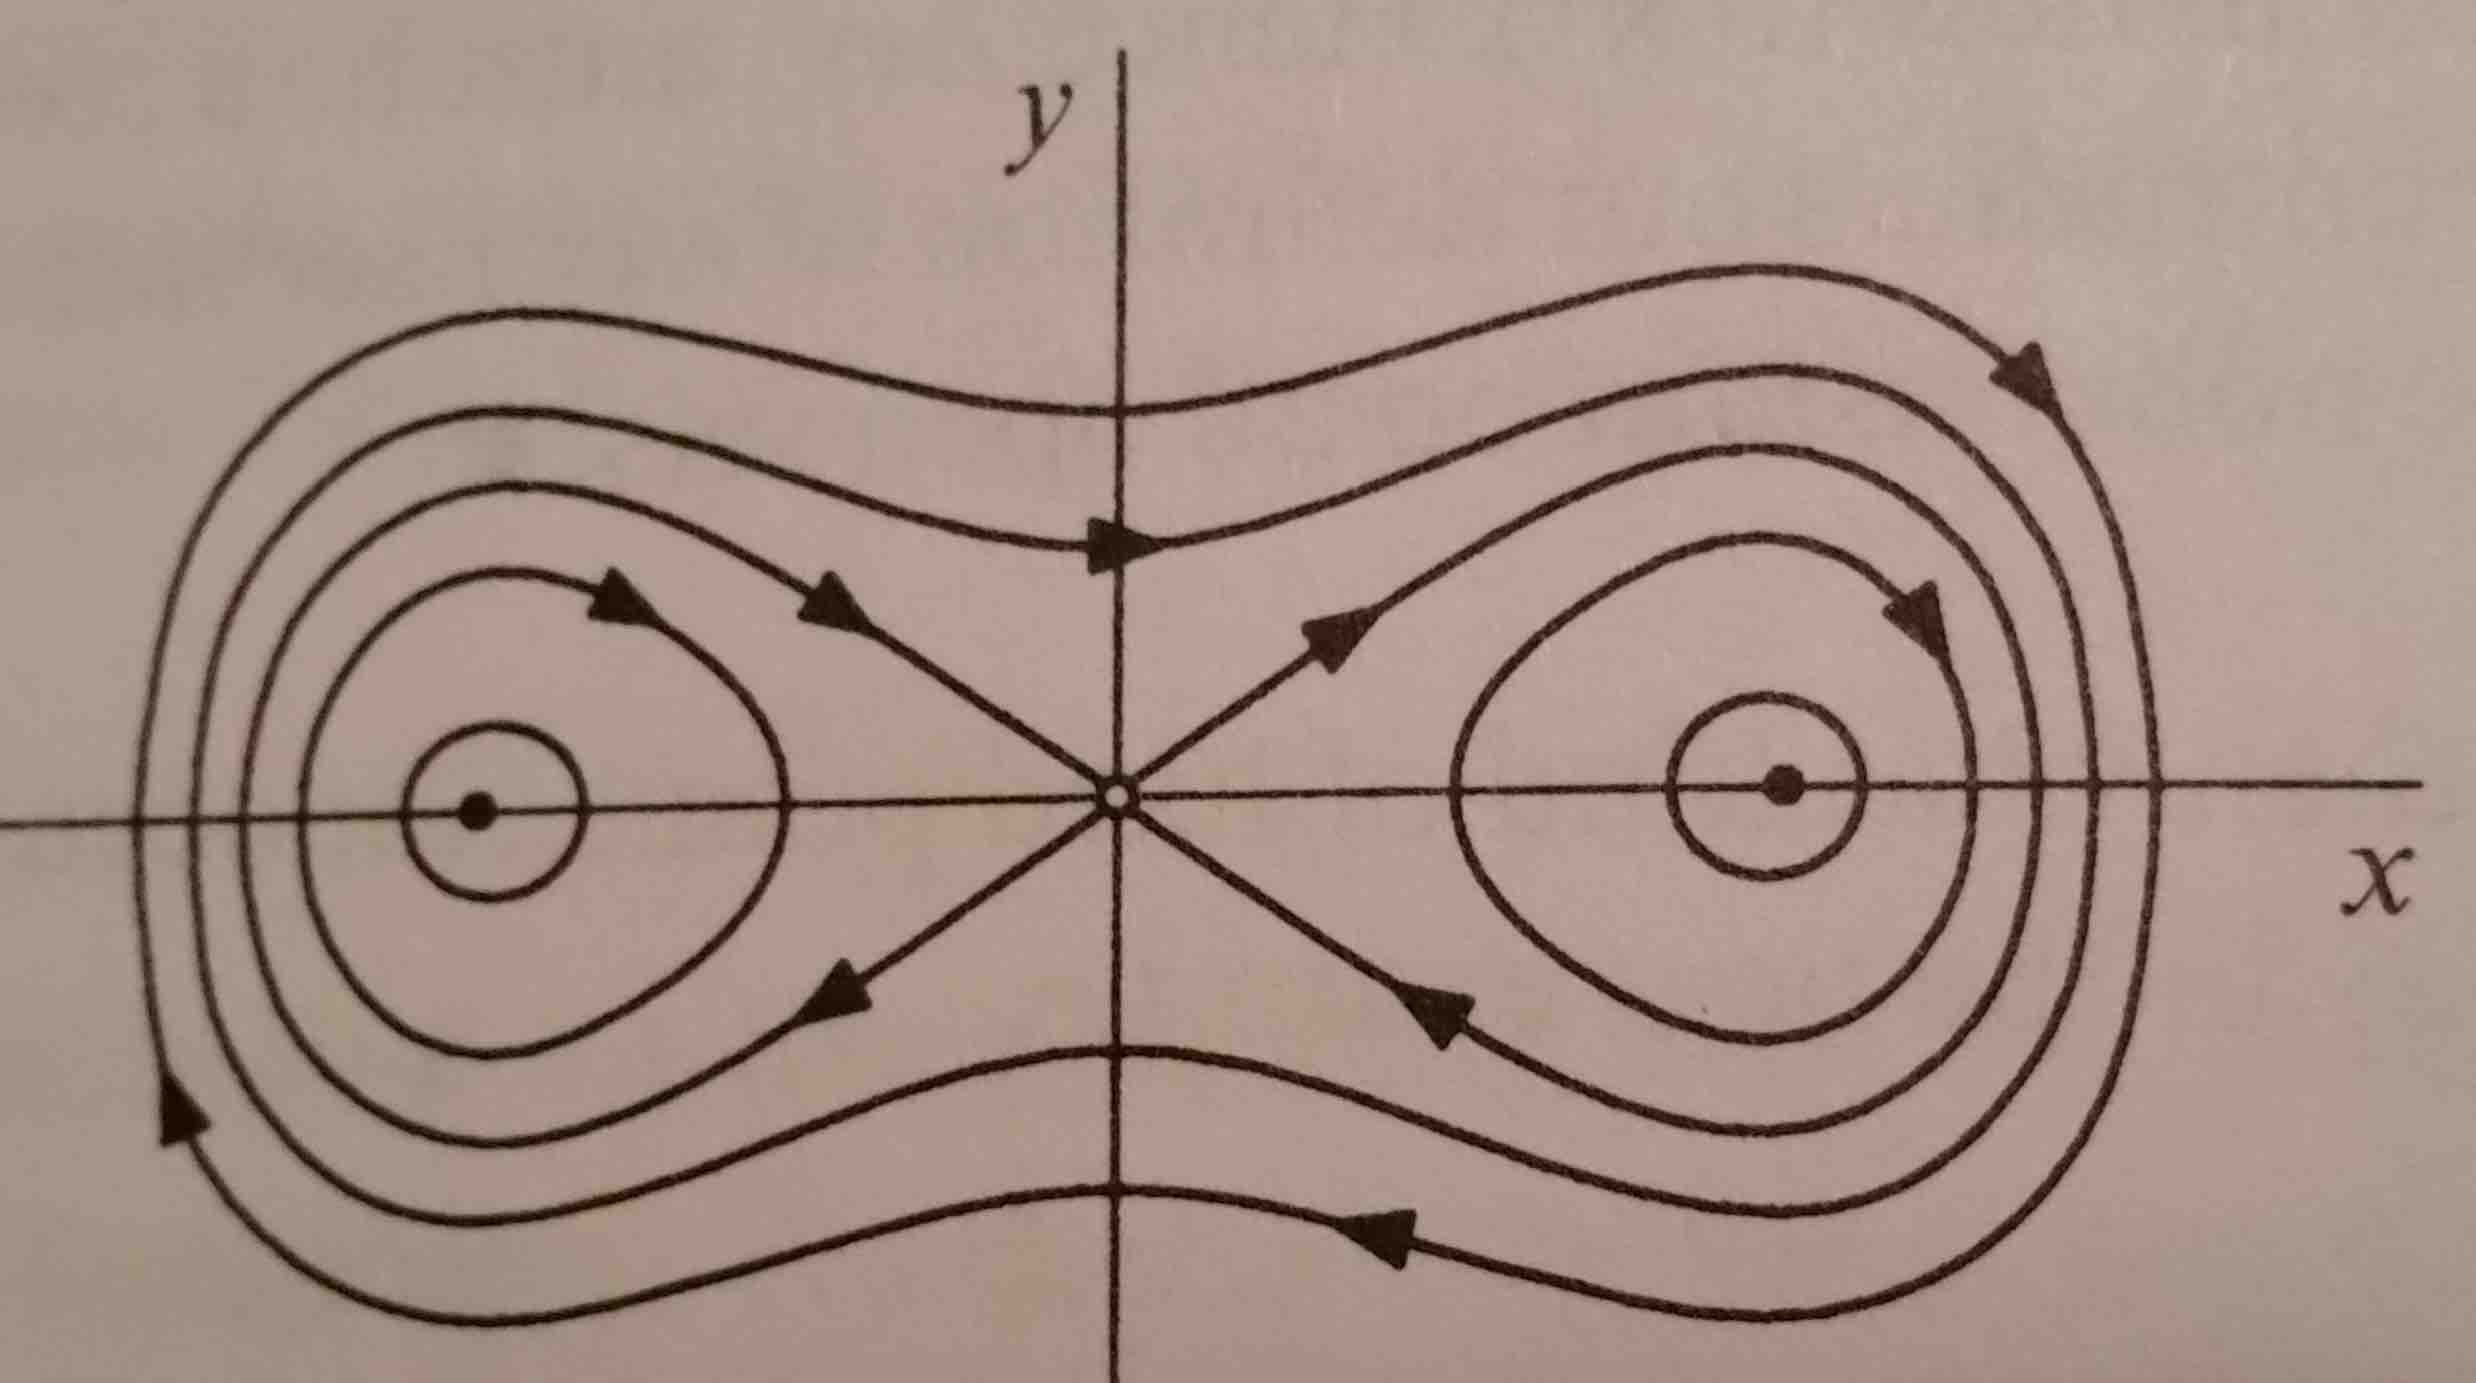
\includegraphics[width = 0.8\textwidth]{ExamplePortrait}
\end{figure}

\end{enumerate}

\end{enumerate}


\end{document}